\section{Deciphering Spanish Gigaword}
\label{decipher_gigaword}
In this section, we describe data and experiment details for deciphering Spanish into English.

\subsection{Data}

In our Spanish-English decipherment experiments, we use half of the Gigaword corpus as monolingual data, and a small amount of parallel data from Europarl for evaluation. We keep only the top 10,000 most frequent word types for both languages and replace all other word types with ``UNK''.  We also exclude sentences with more than 40 tokens as longer sentences significantly slow down the parser\cite{bohnet:2010:PAPERS}  we use. After preprocessing, the size of data for each language is shown in Table \ref{es-en-data}. The Gigaword corpus consists of news articles from different news agencies.  While we use all the monolingual data shown in Table \ref{es-en-data} to learn word embeddings, we only parse the AFP (Agence France-Presse) section of the corpus to extract cipher dependency bigrams and build a plaintext language model. We also use GIZA\cite{GIZA} to align a small amount of parallel data to build a dictionary for decipherment evaluation.

 \begin{table}
 \begin{center}
 \begin{tabular}{ |c|c|c| } \hline
             & Spanish & English \\ \hline
Non Parallel & \multirow{2}{*}{992 million} & \multirow{2}{*}{940 million} \\ 
(Gigaword) & &  \\ \hline
Parallel & \multirow{2}{*}{1.1 million} & \multirow{2}{*}{1.0 million} \\
(Europarl) & &  \\ \hline
 \end{tabular}
 \caption{Size of data in tokens used in Spanish-English decipherment}
 \label{es-en-data}
 \end{center}
 \end{table}

\subsection{Systems}
We implement a baseline system based on the work described in \newcite{dou-knight:2013:EMNLP}. The baseline system performs decipherment on dependency bigrams.Therefore, we use dependency parser to parse AFP section of both Spanish and English version of Gigaword corpus. Since not all dependency relations are shared across the two languages, we do not extract all dependency bigrams. Instead, we only use bigrams with dependency relations in the following list: 

\begin{itemize}
\item Verb-Subject
\item Verb-Noun Object
\item Preposition-Preposition Object
\item Noun-Noun Modifier
\end{itemize}

The baseline uses slice sampling with uniform base distribution during decipherment.

We denote the system that uses our new method as \textbf{Decipher-Embedding}. The system is the same as the baseline except that it uses a base distribution derived from word context similarities.  

For all the systems, language models are built using the SRILM toolkit \cite{srilm}. We use modified Kneyser-Ney \cite{KneserNey95} algorithm for smoothing.


\subsection{Sampling Procedure}
\label{sample_procedure}
In experiments, we find that the iterative sampling method described by \newcite{Dou:2012} helps improve deciphering accuracy. We also find that combining results from different decipherments helps find more correct translations at each iteration. Thus, instead of using a single sampling process, we use 10 different sampling processes at each iteration. The details of the new sampling procedure are provided here:

 \begin{itemize}
  \item Extract dependency bigrams from parsing outputs and collect their counts.
  \item Keep bigrams whose counts are greater than a threshold $\alpha$. Then start 10 different randomly seeded and initialized sampling processes. Perform sampling.
  \item At the end of sampling, extract word translation pairs $(f,e)$ from the final sample. Estimate translation probabilities $P(e|f)$  for each pair. Then construct a translation table by keeping translation pairs $(f,e)$ seen in more than one decipherment and use the average $P(e|f)$ as the new translation probability.
  \item Lower the threshold $\alpha$ to include more bigrams into the sampling process. Start 10 different sampling processes again and initialize the first sample using the translation pairs obtained from the previous step (for each Spanish token f, choose an English token e whose $P(e|f)$ is the highest). Perform sampling again.
  \item Repeat until $\alpha=1$.
\end{itemize}


\subsection{Deciphering Accuracy}
We choose the first 1000 lines of the monolingual Spanish texts as our test data. The data contains 37,505 tokens and 6556 word types. We use type accuracy as our evaluation metric: Given a word type $f$ in Spanish, we find a translation pair $(f,e)$ with the highest average $P(e|f)$ from the translation table learned through decipherment. If the translation pair $(f,e)$ can also be found in a gold translation lexicon $T_{gold}$, we treat the word type $f$ as correctly deciphered. Let $|C|$ be the number of word types correctly deciphered, and $|V|$ be the total number of word types evaluated. We define type accuracy as $\frac{|C|}{|V|}$.

To create $T_{gold}$, we use GIZA \cite{Och:2003:SCV:778822.778824} to align a small amount of Spanish-English parallel text (1 million tokens for each language), and use the lexicon derived from the alignment as our gold translation lexicon. $T_{gold}$ contains a subset of 4408 types seen in the test data, among which, 2878 are also top 5000 frequent word types.

\section{Deciphering Malagasy}
\label{decipher_gigaword}
In this section, we first introduce the Malagasy language, and describe the data used in the experiments; then explain what makes deciphering Malagasy more challenging compared with Spanish, and differences in experiment settings for achieving higher decipherment accuracy.

\subsection{The Malagasy Language}
Malagasy is the official language of Madagascar. It has around 18 million native speakers. Although Madagascar is an African country, Malagasy belongs to the Malayo-Polynesian branch of the Austronesian language family. Malagasy and English have very different word orders. First of all, in contrast to English, which has a subject-verb-object (SVO) word order, Malagasy has a verb-object-subject (VOS) word order. Besides that, Malagasy is a typical head initial language: Determiners precede nouns, while other modifiers and relative clauses follow nouns (e.g. ny ``the'' boky ``book'' mena ``red''). The significant differences in word order pose great challenges for decipherment.


\subsection{Data}
We list the size of both monolingual and parallel data used in this experiment in Table \ref{mlg-en-data}. The data used in this experiment is released from previous work by \newcite{dou-vaswani-knight:2014:EMNLP2014}. The monolingual data in Malagasy contains news data collected from various local websites. The English monolingual data contains Gigaword and additional 300 million tokens of news on Africa. The parallel data is collected from GlobalVoices, a multilingual news website, where volunteers translate news into different languages. The parallel data is used to build a dictionary for evaluating decipherment accuracy. 

 \begin{table}
 \begin{center}
 \begin{tabular}{ |c|c|c| } \hline
             & Malagasy & English \\ \hline
\multirow{2}{*}{Non Parallel} & 16 million & 1.2 billion\\ 
& (Web) & (Gigaword + Web) \\ \hline
Parallel & \multirow{2}{*}{2.0 million} & \multirow{2}{*}{1.8 million} \\
(GlobalVoices) & &  \\ \hline
 \end{tabular}
 \caption{Size of data in tokens used in Malagasy-English decipherment}
 \label{mlg-en-data}
 \end{center}
 \end{table}
 
\subsection{Systems}
The baseline system is the same as the baseline used in Spanish-English decipherment experiments. We use data provided in previous work \cite{dou-vaswani-knight:2014:EMNLP2014} to build a Malagasy dependency parser. For English, we use Turbo parser trained on Penn Treebank \cite{TurboParser}.  

Since the Malagasy parser doesn't predict dependency relation types, we use head-child part-of-speech (POS) tag patterns to select a subset of dependency bigrams for decipherment. We list the selected POS tag patterns in Table \ref{mlg-en-dep-type}.

%
 \begin{table}
 \begin{center}
 \begin{tabular}{ |c|c| } \hline
          Head POS & Child POS \\ \hline
Verb & Noun \\ \hline
Verb & Proper Noun \\ \hline
Verb & Person Pronoun \\ \hline
Preposition & Noun \\ \hline
Preposition & Proper Noun \\ \hline
Noun 2 & Adjective \\ \hline
Noun 3 & Determiner \\ \hline
Noun & Verb Particle \\ \hline
Noun 2 & Verb Noun \\ \hline
Noun & Cardinal Number \\ \hline
 \end{tabular}
 \caption{Head-Child POS patterns used in decipherment}
 \label{mlg-en-dep-type}
 \end{center}
 \end{table}
%

\subsection{Sampling Procedure}
We use the same sampling protocol designed for Spanish-English decipherment. However, in experiments, we find out that simply using viterbi decoding to initialize the first sample does not work as well as in deciphering Spanish. Therefore, in addition to using Viterbi decoding, we also initialize the base distribution to the base distribution of previous decipherment run that produces highest decipherment accuracy.

\subsection{Results}
During decipherment, we gradually increase the size of Spanish texts and compare the learning curves of three deciphering systems in Figure \ref{curve}.

 \begin{figure}[!ht]
  \centering
  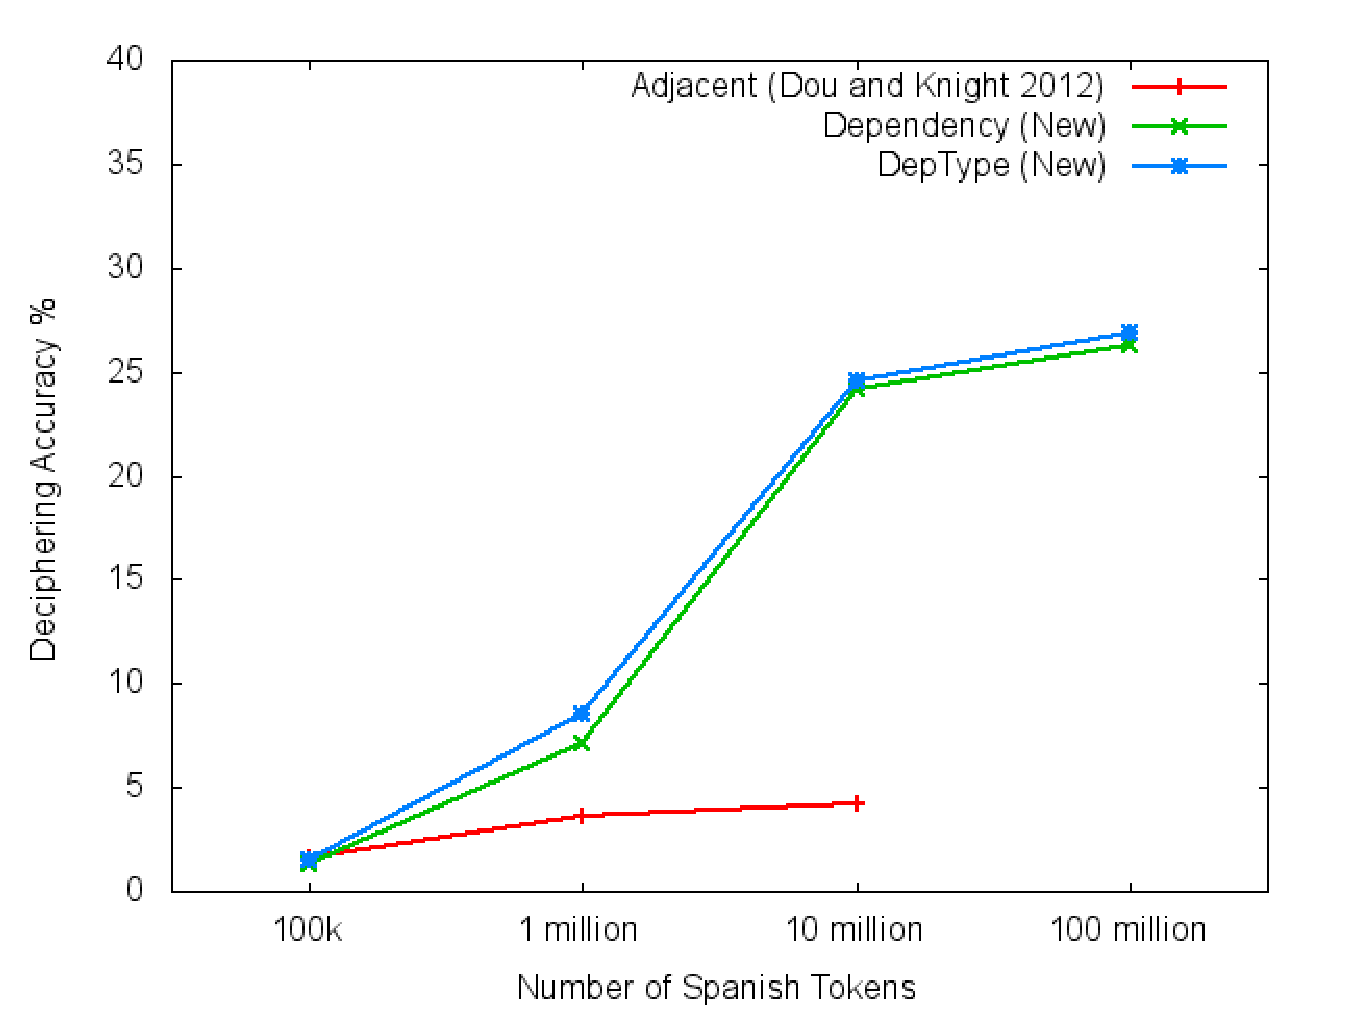
\includegraphics[width=3.3in,height=2.4in]{curve}
  \caption{Learning curves for Malagasy-English decipherment.}
\label{mlg-en-curve}
\end{figure}

 \begin{figure}[!ht]
  \centering
  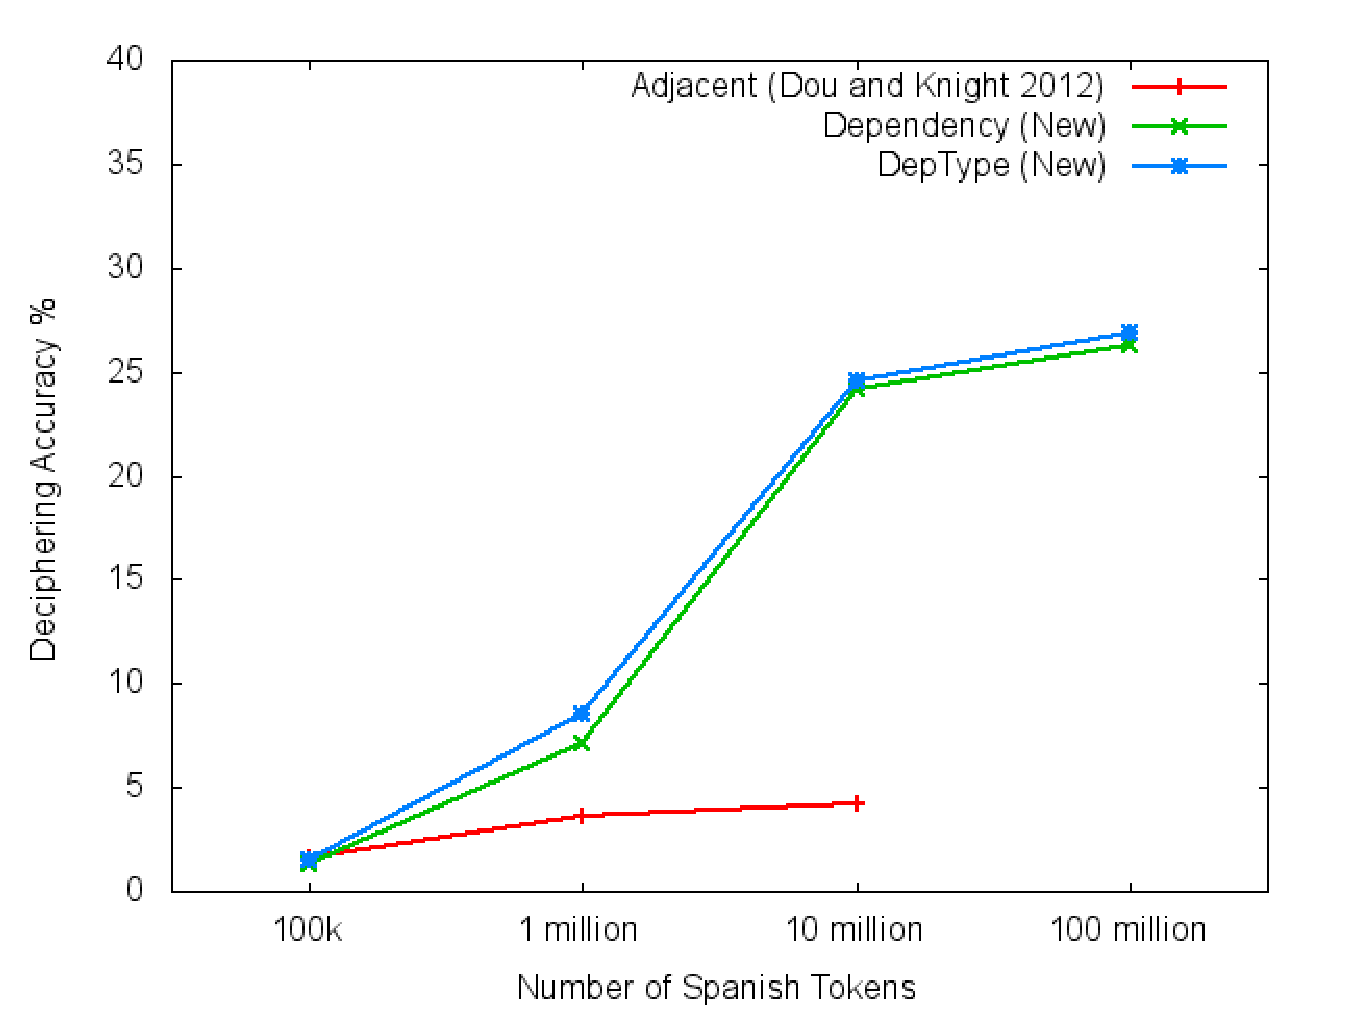
\includegraphics[width=3.3in,height=2.4in]{curve}
  \caption{Learning curves for Spanish-English decipherment.}
\label{es-en-curve}
\end{figure}

With 100k tokens of Spanish text, the performance of the three systems are similar. However, the learning curve of Adjacent plateaus quickly, while those of the dependency based systems soar up as more data becomes available and still rise sharply when the size of Spanish texts increases to 10 million tokens, where the DepType system improves deciphering accuracy of the Adjacent system from 4.2\% to 24.6\%. In the end, with 100 million tokens, the accuracy of the DepType system rises to 27.0\%. The accuracy is even higher (41\%), when evaluated against the top 5000 frequent word types only.




